\chapter{Diseño e implementación} % Main chapter title

\label{Chapter3} % Change X to a consecutive number; for referencing this chapter elsewhere, use \ref{ChapterX}

\definecolor{mygreen}{rgb}{0,0.6,0}
\definecolor{mygray}{rgb}{0.5,0.5,0.5}
\definecolor{mymauve}{rgb}{0.58,0,0.82}

%%%%%%%%%%%%%%%%%%%%%%%%%%%%%%%%%%%%%%%%%%%%%%%%%%%%%%%%%%%%%%%%%%%%%%%%%%%%%
% parámetros para configurar el formato del código en los entornos lstlisting
%%%%%%%%%%%%%%%%%%%%%%%%%%%%%%%%%%%%%%%%%%%%%%%%%%%%%%%%%%%%%%%%%%%%%%%%%%%%%
\lstset{ %
  backgroundcolor=\color{white},   % choose the background color; you must add \usepackage{color} or \usepackage{xcolor}
  basicstyle=\footnotesize\ttfamily,        % the size of the fonts that are used for the code
  breakatwhitespace=false,         % sets if automatic breaks should only happen at whitespace
  breaklines=true,                 % sets automatic line breaking
  captionpos=b,                    % sets the caption-position to bottom
  commentstyle=\color{mygreen},    % comment style
  deletekeywords={...},            % if you want to delete keywords from the given language
  %escapeinside={\%*}{*)},          % if you want to add LaTeX within your code
  %extendedchars=true,              % lets you use non-ASCII characters; for 8-bits encodings only, does not work with UTF-8
  %frame=single,	                % adds a frame around the code
  keepspaces=true,                 % keeps spaces in text, useful for keeping indentation of code (possibly needs columns=flexible)
  keywordstyle=\color{blue},       % keyword style
  language=Python,                 % the language of the code
  %otherkeywords={*,...},           % if you want to add more keywords to the set
  numbers=left,                    % where to put the line-numbers; possible values are (none, left, right)
  numbersep=5pt,                   % how far the line-numbers are from the code
  numberstyle=\tiny\color{mygray}, % the style that is used for the line-numbers
  rulecolor=\color{black},         % if not set, the frame-color may be changed on line-breaks within not-black text (e.g. comments (green here))
  showspaces=false,                % show spaces everywhere adding particular underscores; it overrides 'showstringspaces'
  showstringspaces=false,          % underline spaces within strings only
  showtabs=false,                  % show tabs within strings adding particular underscores
  stepnumber=1,                    % the step between two line-numbers. If it's 1, each line will be numbered
  stringstyle=\color{mymauve},     % string literal style
  tabsize=2,	                   % sets default tabsize to 2 spaces
  title=\lstname,                  % show the filename of files included with \lstinputlisting; also try caption instead of title
  morecomment=[s]{"""}{"""},
  morekeywords={self,as,assert,nonlocal,with,yield,self,True,False,None,,object,type,isinstance,copy,deepcopy,zip,enumerate,reversed,list,set,len,dict,tuple,range,xrange,append,execfile,real,imag,reduce,str,repr,ode,fsolve,sqrt,exp,sin,cos,arctan,arctan2,arccos,pi, array,norm,solve,dot,arange,isscalar,max,sum,flatten,shape,reshape,find,any,all,abs,plot,linspace,legend,quad,polyval,polyfit,hstack,concatenate,vstack,column_stack,empty,zeros,ones,rand,vander,grid,pcolor,eig,eigs,eigvals,svd,qr,tan,det,logspace,roll,min,mean,cumsum,cumprod,diff,vectorize,lstsq,cla,eye,xlabel,ylabel,squeeze},
  inputencoding=utf8,              % usa UTF-8 para interpretar el código
  literate=%
    {á}{{\'a}}1 {é}{{\'e}}1 {í}{{\'i}}1 {ó}{{\'o}}1 {ú}{{\'u}}1
    {Á}{{\'A}}1 {É}{{\'E}}1 {Í}{{\'I}}1 {Ó}{{\'O}}1 {Ú}{{\'U}}1
    {ñ}{{\~n}}1 {Ñ}{{\~N}}1 {¿}{{\textquestiondown}}1 {¡}{{\textexclamdown}}1
}

%----------------------------------------------------------------------------------------
%	INTRODUCCIÓN AL CAPÍTULO
%----------------------------------------------------------------------------------------

En este capítulo se explica cómo se han utilizado los modelos y herramientas de inteligencia artificial descritos en los capítulos anteriores junto con otras técnicas de programación para crear una aplicación que permite generar tanto el contenido como las imágenes de un email de forma automática. Se detallan desde los primeros intentos en explorar las posibles soluciones, hasta la forma como se terminaron construyendo los módulos de generación de texto, imagen y la interfaz gráfica.

%----------------------------------------------------------------------------------------
%	SECTION 1
%----------------------------------------------------------------------------------------

\section{Aproximación inicial a la solución y diseño de plantillas}

La ideación de la solución comenzó con experimentos básicos en los que se le pedía a ChatGPT construir emails en HTML brindándole una plantilla a través de la interfaz de OpenAI. El propósito de estos experimentos era probar qué tan bueno podía ser un gran modelo de lenguaje al crear un email a partir de una plantilla. En la figura~\ref{fig:PruebaChatGPT} se puede ver el resultado (ignorar para este caso la imagen, ya que únicamente se estaba testeando la generación de texto). En el lado izquierdo se puede observar cómo se ve la plantilla brindada a ChatGPT con un mensaje inventado que debía ser modificado por el modelo. Cabe resaltar que se le dio la plantilla como código HTML. Posteriormente, se le dio la siguiente instrucción:

\begin{quote}
``Quiero que mantengas las imágenes, pero cambia el contenido del email. Cámbialo para que sea un campaña de venta de tarjeta de crédito: Adquiere tu tarjeta de crédito Visa Signature con S/ 20 000 de línea de crédito. Tendrás múltiples beneficios (colocar los beneficios en viñetas): descuentos en restaurantes, pases a las salas vip de aeropuertos, cuotas sin intereses, tasa preferencial de 20\%.''
\end{quote}

Como se observa en el resultado 1 de la figura~\ref{fig:PruebaChatGPT}, el modelo cambia correctamente el mensaje y brinda un título y párrafos coherentes con lo solicitado. Sin embargo no termina de generar todo el contenido por la gran extensión de la parte legal de la plantilla. En vez de brindar el email completo, el modelo colocó este mensaje dentro del código: \texttt{<!-- Resto del contenido... -->}. 

Se le pidió al modelo brindar el resto del código que debía ser colocado en vez de ese mensaje y generó código que se tuvo que copiar y pegar manualmente para obtener el resultado 2 de la figura~\ref{fig:PruebaChatGPT}. En esta segunda iteración se logró un email más completo. Sin embargo, el modelo colocó un texto legal más resumido, inventó un nombre para la página de Facebook de la compañía distinto al brindado en la plantilla y también creó un URL ficticio de la web oficial.

\begin{figure}[!htpb]
     \centering
     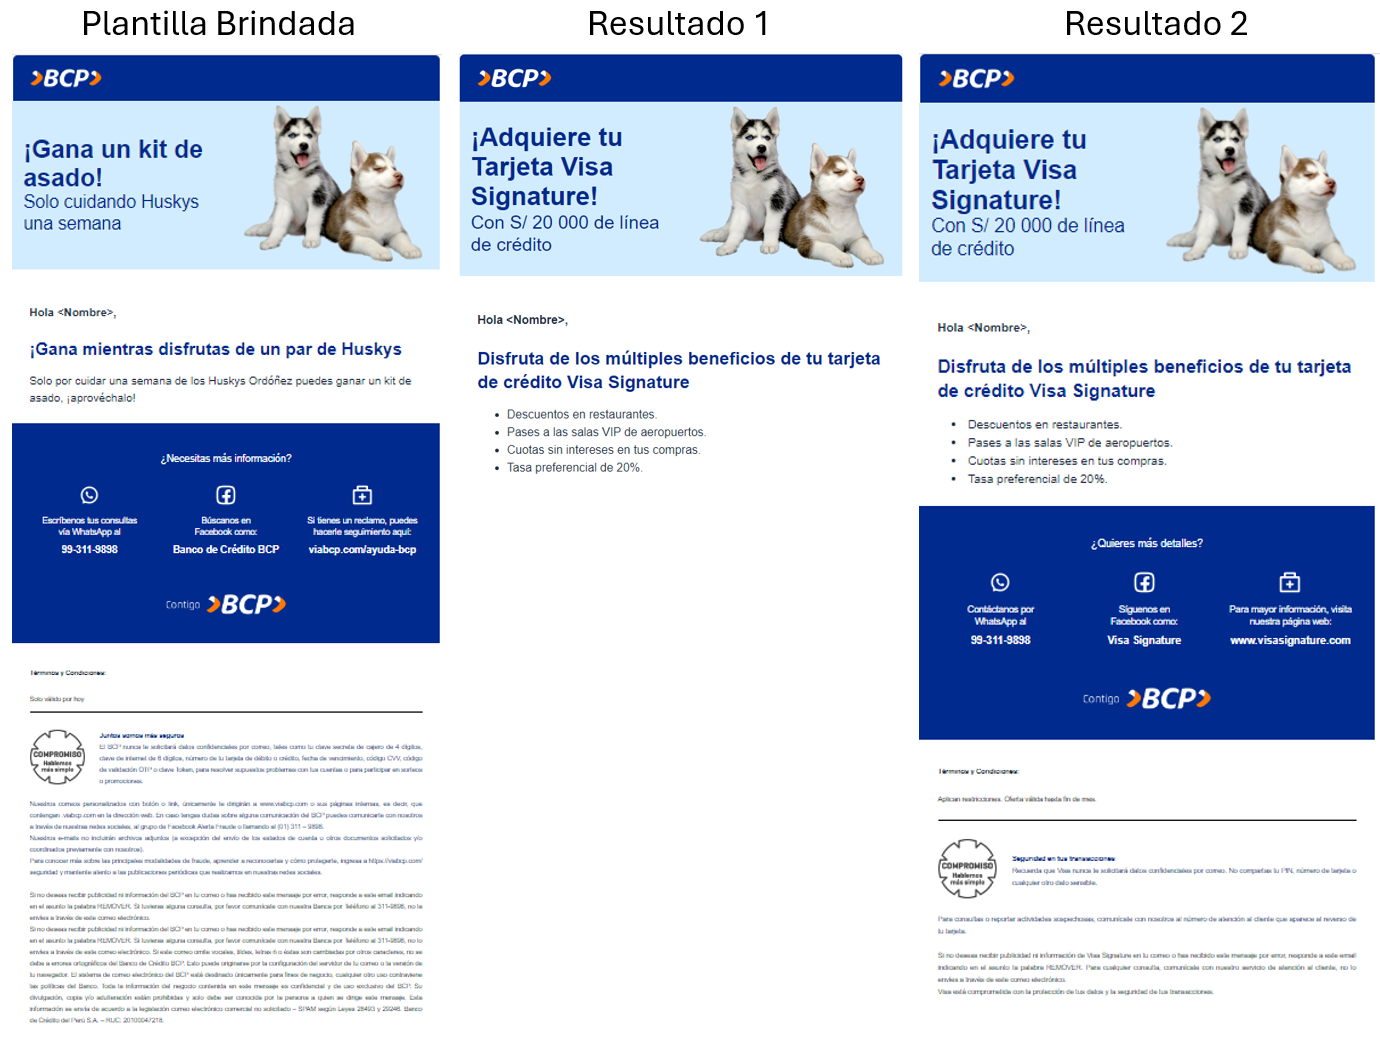
\includegraphics[width=1\textwidth]{./Figures/Prueba_Inicial_Chatgpt.png}
    \caption{Prueba realizada con ChatGPT.}
    \label{fig:PruebaChatGPT}
\end{figure}

Con esta experiencia se sacaron varias conclusiones. Una de ellas es que los LLMs sí son capaces de entender HTML y modificar su contenido coherentemente, pero tienden a limitar la cantidad de \textit{tokens} que brindan como \textit{output}, por lo que pueden arrojar emails incompletos. 

Adicionalmente, hay partes como el legal o la web de la empresa, que ya están definidos y no se necesita que un LLM las modifique. Incluso su modificación es perjudicial. Darle la oportunidad al LLM de que edite un correo completo incrementa la posibilidad de que se cambien partes del email que no se deben alterar como los colores de marca, la maquetación, los datos de contacto, entre otros detalles.

Por otro lado, el costo de usar un LLM está relacionado a la cantidad de \textit{tokens} de \textit{input} y \textit{output}, por lo que brindarle una plantilla con todo el texto legal y pedirle que retorne el mismo texto sin modificaciones no es eficiente en términos de procesamiento ni de costos.

Este análisis inicial condujo a la decisión de optar por una solución más estructurada mediante la creación de clases y funciones que utilicen código HTML de plantillas predefinidas sin necesidad de que el gran modelo de lenguaje las tenga que conocer a detalle. Lo único que es necesario que el LLM genere es el contenido variable del email, que posteriormente es insertado en las plantillas.

Para lograr este planteamiento, la primera tarea consistió en comprender la estructura de un email modelo proporcionado por la empresa e identificar todos los elementos que lo componen. Entre ellos están los siguientes: la cabecera, el cuerpo principal, el cierre y la sección legal. El detalle de la estructura de un email modelo se presentó en el capítulo anterior en las figuras~\ref{fig:EjConsumo} y~\ref{fig:EjBEX}.

Poder separar los elementos del email permitió identificar cuáles se deben modificar de los que no. Los elementos que no se modifican se dejan como parte del código de las plantillas, mientras que las partes que sí cambian son manejadas como \textit{inputs} para la creación de clases. 

Se crearon 2 objetos principales que son los encargados de recibir los \textit{inputs} del contenido del email e insertarlos dentro de las plantillas para obtener el HTML final. A estos objetos se los denominó \texttt{Email\_html} y \texttt{Contenido\_principal}. A su vez, se crearon clases secundarias para manejar el contenido que se puede agregar al email de forma opcional: \texttt{Contenido\_extra}, \texttt{Legal\_extra}, \\ \texttt{Seccion\_iconos}, \texttt{Recuadro\_premio} y \texttt{Recuadro\_lista}.

En la figura~\ref{fig:Diagrama_clases} se encuentra un diagrama que ayuda a entender mejor la relación entre estas clases y los elementos que contiene cada una. Existen clases que son \textit{inputs} de otras más generales. El objeto que engloba a todas y cuya instancia representa un email completo con todos sus elementos es la clase \texttt{Email\_html}. 


\begin{figure}[!htpb]
    \centering
    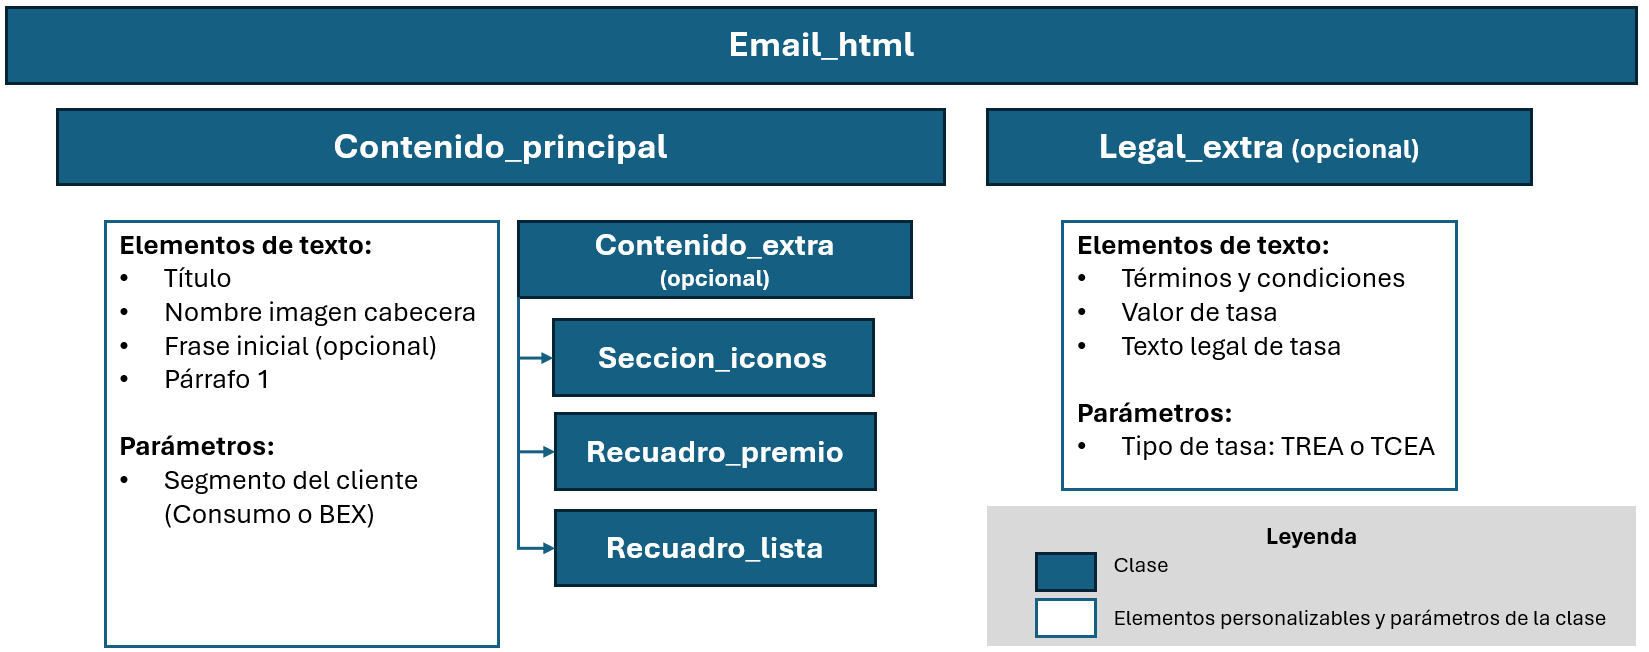
\includegraphics[width=0.95\linewidth]{Figures/Diagrama_clases.png}
    \caption{Diagrama de clases y sus elementos.}
    \label{fig:Diagrama_clases}
\end{figure}

En la figura~\ref{fig:DefinicionClase} se puede observar la estructura general que se ha seguido para definir una clase.

\begin{figure}[!htpb]
    \centering
    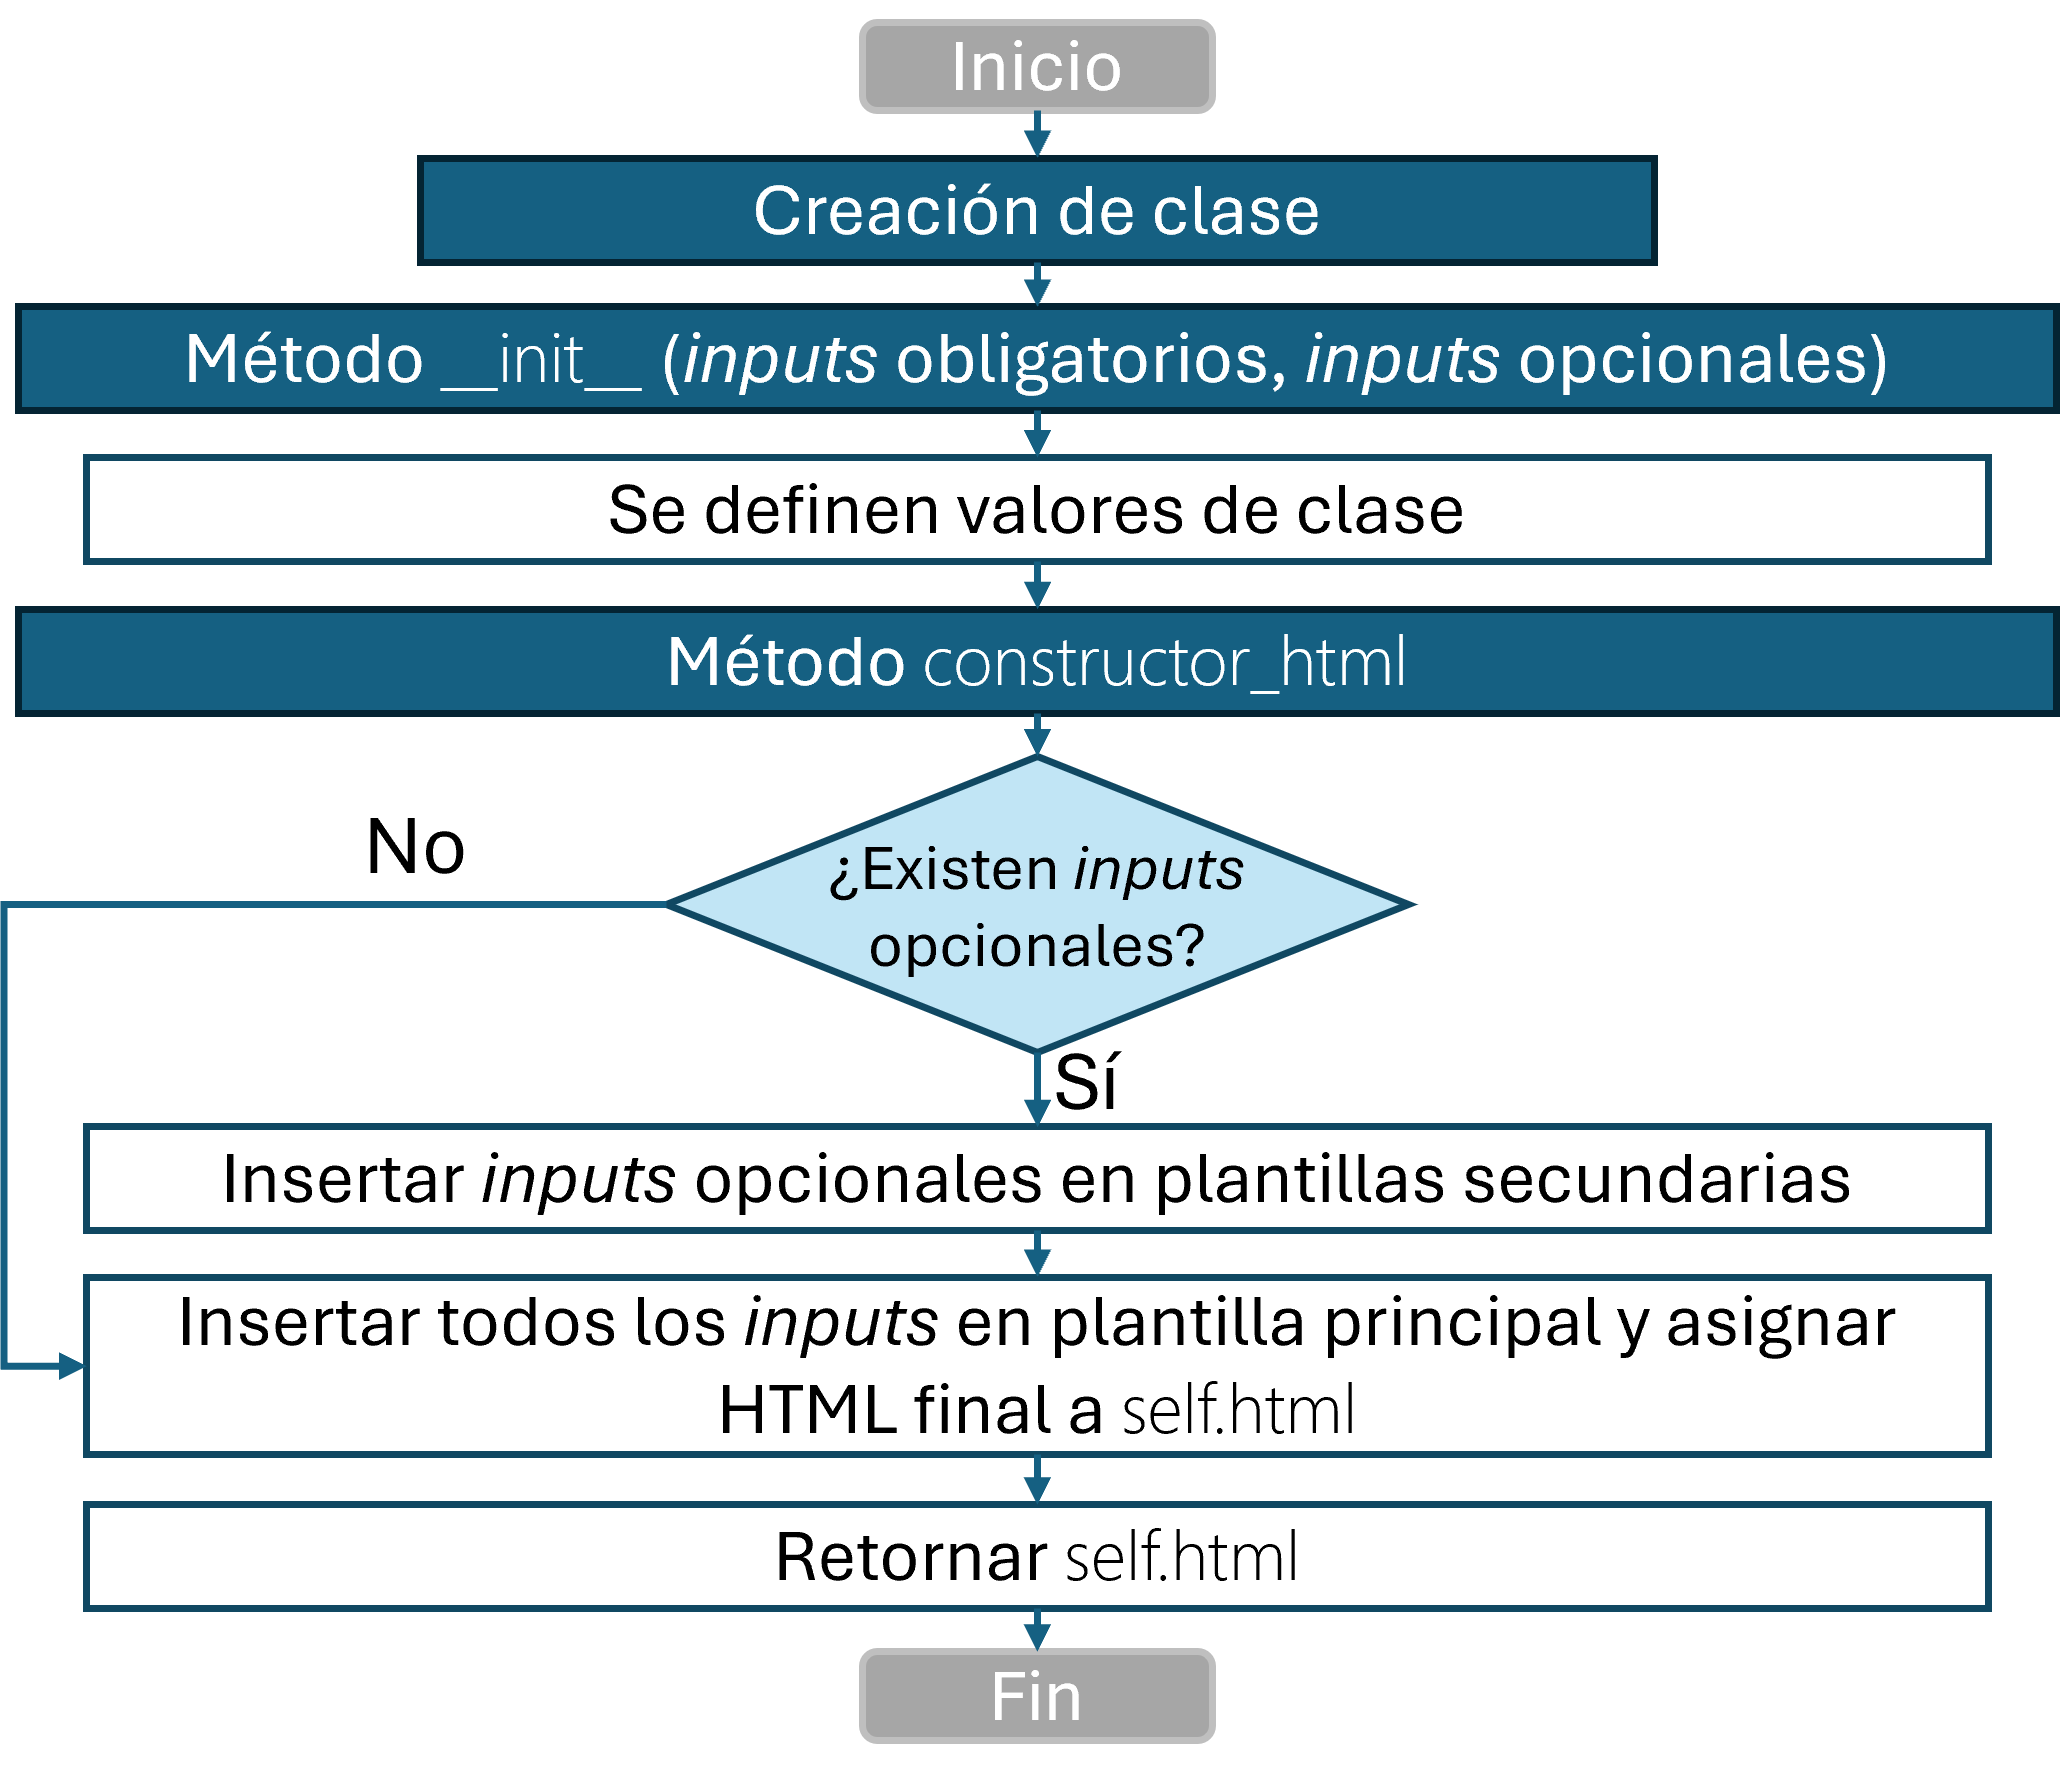
\includegraphics[width=0.7\linewidth]{Figures/Flujo_creacion_clase.png}
    \caption{Flujo de la creación de una clase HTML.}
    \label{fig:DefinicionClase}
\end{figure}

Como se muestra en el diagrama, al inicializar la clase se le comparten ciertos parámetros que son obligatorios y otros que son opcionales. Por ejemplo, en el caso de la clase \texttt{Contenido\_principal}  los obligatorios son \texttt{segmento\_cliente}, \\ \texttt{img\_cabecera}, \texttt{titulo\_1}, \texttt{titulo\_2} y \texttt{parrafo\_1}. Estos son los mínimos elementos necesarios para generar un email coherente. En específico, el parámetro \texttt{segmento\_cliente} es el que indica si se usará la plantilla de un email para clientes BEX o Consumo. Por otro lado, los parámetros opcionales para esta clase son la \texttt{frase\_inicial} y una instancia de la clase \texttt{Contenido\_extra}.

Una vez que se inicializa la clase, se utiliza el método \texttt{constructor\_html} para poder llamar a las plantillas correspondientes e insertarles el contenido. Todas las plantillas utilizan \textit{string format} para poder insertar contenido de variables dentro del texto y están definidas en el módulo \texttt{mod\_string\_format.py}. Específicamente la clase \texttt{Contenido\_principal} utiliza las siguientes plantillas: \\ \texttt{contenido\_consumo}, \texttt{contenido\_bex}, \texttt{frase\_inicial} . 

Con la creación de estas plantillas y clases que se encargan de armar el HTML de forma más ordenada, el siguiente paso fue conseguir que el gran modelo de lenguaje pueda trabajar con estas clases y brindarles los \textit{inputs} adecuados para que el email pueda ser generado. Esta parte del desarrollo se explica en la siguiente sección.

%-------------------------------------------------------------------------------------------------------------
%-------------------------------------------------------------------------------------------------------------

\section{Generación del contenido del email con LLMs}

Para lograr que el modelo de lenguaje pueda utilizar las clases creadas se decidió optar por crear un agente LLM. Como se explicó en la sección~\ref{sec:LagchainAgentes}, los agentes tienen la particularidad de que se les pueden brindar herramientas (\textit{tools}) para que realicen acciones y ejecuten código, no solo generar texto, que era lo que se necesitaba para este proyecto. El agente puede ejecutar una función que reciba como parámetros los \textit{inputs} del contenido del email y los utilice para crear las instancias de clases necesarias.

Para la creación del agente basado en un modelo de lenguaje, se decidió utilizar LangChain \cite{langchain}. A través de LangChain, se configuró el acceso a la API de OpenAI que permite realizar solicitudes a grandes modelos de lenguaje como GPT4o-mini. Además, LangChain ya proporciona plantillas y estructuras para poder generar agentes con \textit{tools} personalizados. Para este trabajo, se decidió utilizar un agente ReAct \cite{yao2022react}, que está instruido para razonar antes de realizar una acción. Seguir esta secuencia lógica le permite al LLM detenerse a analizar qué \textit{tool} usar y cómo usarlo antes de ejecutar cualquier función.

\subsection{Creación de la función create\_email}

La función \texttt{create\_email} es la que se le asignó al agente LLM como \textit{tool} para que ejecute y es importante porque es la conexión entre el modelo y las clases y plantillas creadas. Inicialmente se hicieron pruebas creando una función que recibía varios parámetros (uno por elemento del email), pero el modelo de agente ReAct que se estaba usando fallaba al tener que brindar más de un parámetro. Así que se optó por crear una función con un solo parámetro de entrada: un texto en formato JSON que contenga todos los elementos del email.

Este texto se convierte a JSON dentro de la función y sus elementos se van utilizando para inicializar las clases correspondientes. El formato JSON resultó ser bastante conveniente ya que permite decidir qué elementos enviar y cuáles no, algo útil al momento de trabajar con los \textit{inputs} opcionales del email. Para el manejo de estos campos opcionales, se incluyó dentro de la función validaciones para adaptar la inicialización de las clases dependiendo si se envían estos campos o no. En la figura~\ref{fig:createEmail} se puede ver la estructura de la función \texttt{create\_email} con más detalle.

\begin{figure}[!htpb]
    \centering
    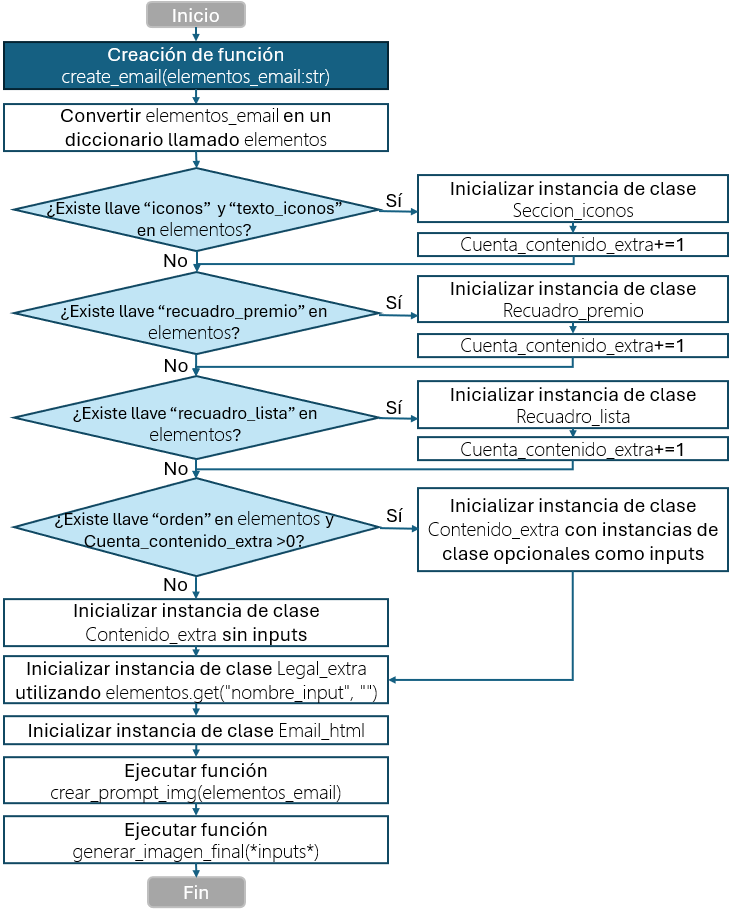
\includegraphics[width=1\linewidth]{Figures/Flujo_create_email.png}
    \caption{Flujo de la función \texttt{create\_email}.}
    \label{fig:createEmail}
\end{figure}

Como se puede observar, la variable \texttt{elementos} es un diccionario que se crea a partir del JSON y es la que contiene todos los \textit{inputs} del contenido del email. Existen algunos elementos como \texttt{iconos} o \texttt{tcea\_trea} que son opcionales y se usan estructuras \texttt{if} o el método \texttt{.get} para validar si se enviaron. Al usar \texttt{.get}, en caso de que no se encuentren, se deja su valor como un \texttt{string} vacío, que no afecta el contenido del HTML al insertarse.

La función \texttt{create\_email} contiene también un llamado a otras funciones que generan la imagen de cabecera. Estas serán explicadas en la sección~\ref{sec:GeneracionImg}. Por el momento, lo importante es comentar que dentro del JSON de \textit{input} ya se recibe el nombre de la imagen de cabecera que se incrusta en el HTML. Este se pasa como \textit{input} a la función \texttt{generar\_imagen\_final} para que la imagen a ser generada sea guardada con ese mismo nombre.


\subsection{Creación de las plantillas del \textit{prompt}}

Una parte fundamental al momento de trabajar con grandes modelos de lenguaje es explicarles en detalle lo que se espera que hagan. Esto se logra creando buenas plantillas de \textit{prompts}. Cuando se crea un agente, se necesita más de un \textit{prompt}. Existe uno principal, que es el que le explica al modelo cuál será su rol y sus tareas principales. Luego existe otro por cada \textit{tool} que se le brinde, que explica para qué sirve la herramienta y cómo utilizarla correctamente.

A continuación, se presenta el \textit{prompt} principal del agente que detalla el rol o tarea general que debe cumplir. También es aquí donde se inserta el contenido del email que brinda el usuario.

\begin{quote}
``Ayuda a crear el html para un email considerando este contenido y especificaciones:

Contenido del email: \texttt{\{contenido\}}

Si recibes un error, intenta nuevamente asegurándote de enviar el json en el formato correcto.''
\end{quote}

El segundo \textit{prompt} creado es el del \textit{tool} que explica cómo usar la función \\ \texttt{create\_email}. Este es mucho más extenso porque da bastante detalle sobre cómo estructurar el contenido del email en cada llave del JSON. En el apéndice~\ref{AppendixA} se encuentra el \textit{prompt} completo, pero se puede resumir en los siguientes pasos:

\begin{itemize}
    \item Se explica para qué sirve la herramienta \texttt{create\_email}.
    \item Se informa que el \textit{input} de la función es un texto en formato JSON.
    \item Se enlistan los elementos del JSON que son obligatorios y los que son opcionales.
    \item Se detalla qué incluir en el contenido de cada elemento.
    \item Se agregan instrucciones sobre qué términos se debe evitar mencionar. 
    \item Se explica cómo manejar campos personalizables (aquellos que permiten a la empresa luego adaptar ciertas partes del email a cada cliente, como por ejemplo su nombre).
    \item Se refuerza que se debe enviar el \textit{prompt} en formato JSON sin olvidar separar los elementos con comas.
\end{itemize} 

Este enfoque asegura que el contenido generado esté alineado con los requerimientos específicos de las clases HTML creadas y de las necesidades del usuario. Algo interesante a resaltar es que en ambos \textit{prompts} se repite varias veces que el \textit{input} debe ser brindado en formato JSON, ya que equivocarse en el formato es un error común en los modelos. Repetir esta instrucción ha ayudado a disminuir la probabilidad de ocurrencia de este error.


\subsection{Elección del modelo LLM}

Otra decisión de diseño fue elegir qué modelo LLM utilizar. Inicialmente, se realizaron pruebas con el modelo GPT-3.5 Turbo para generar los emails en HTML. Sin embargo, este modelo mostró limitaciones al entregar respuestas en formato JSON, un aspecto crítico para enviar correctamente los \textit{inputs}. 

Adicionalmente, su redacción del contenido del email tampoco era óptimo ya que repetía palabras que se le brindaban en el \textit{prompt}. Por ejemplo, si se colocaba ``Resalta la exclusividad de esta tarjeta de crédito ...'', a veces ofrecía respuestas como ``Resaltamos nuestra tarjeta más exclusiva ...'', frase que no constituye una expresión natural.

Debido a estos inconvenientes, apenas se lanzó el modelo GPT-4o Mini, se optó por adoptar este modelo y se obtuvieron mejores resultados en cuanto a precisión y formato. Algo que hace al modelo GPT-4o Mini especialmente atractivo es su avanzada capacidad a un costo significativamente menor. En comparación, GPT-4o Mini tiene un precio de \$ 0,15 por millón de \textit{tokens} de entrada y \$ 0,60 por millón de \textit{tokens} de salida, mientras que GPT-3.5 Turbo cuesta \$ 0,50 por millón de \textit{tokens} de entrada y \$ 1,50 por millón de \textit{tokens} de salida \cite{OpenAI2024Pricing}. Esta diferencia de costos, junto con la mejora en el rendimiento, hizo de GPT-4o Mini la opción ideal para este proyecto.

Otro parámetro que se decidió utilizar es una temperatura de 1, lo que permite generar resultados diversos cada vez que se ejecuta la inteligencia artificial con los mismos \textit{inputs}. Esto ayuda a que se le puedan brindar al usuario opciones variadas del email. También evita que el modelo se limite a repetir palabras empleadas en el contenido del \textit{prompt}.

%-------------------------------------------------------------------------------------------------------------
%-------------------------------------------------------------------------------------------------------------

\section{Generación de imágenes con Stable Diffusion}
\label{sec:GeneracionImg}

Se puede dividir el proceso de generación de imágenes de este trabajo en tres pasos:
\begin{itemize}
    \item Generar el \textit{prompt} de la imagen: se debe crear un texto descriptivo de la imagen que se desea crear.
    \item Generar la imagen en bruto: se debe compartir el texto descriptivo al API de StabilityAI para generar la imagen.
    \item Remover el fondo de la imagen: se debe remover el fondo para que la imagen tenga transparencia y pueda ser colocada encima del fondo de color del HTML.
\end{itemize}

En las siguientes subsecciones se detalla cómo se realizaron cada uno de estos pasos.
\pagebreak
\subsection{Generación del \textit{prompt} de la imagen}

Para automatizar por completo el proceso, el \textit{prompt} de la imagen a crear se realiza mediante el uso de un segundo agente LLM, configurado de manera similar al utilizado para crear el texto del email. Este se encarga de revisar el contenido generado previamente por el primer agente. A partir de esta revisión, crea un \textit{prompt} que describe la imagen más adecuada para acompañar dicho contenido.

Cabe resaltar que en un primer momento se intentó generar esta descripción de la imagen dentro del proceso del primer agente. Sin embargo, se necesitaban brindar varias instrucciones para que la imagen descrita sea adecuada. Al agregar todo este texto adicional dentro del \textit{prompt} del primer agente, se volvía muy complejo que el modelo pueda obedecer todas las instrucciones. Tras varias pruebas se evidenció que entre más tareas se le pida realizar a un agente, existe mayor posibilidad de que omita alguna indicación o de que la lleve a cabo de forma incorrecta.

En el \textit{prompt} de este segundo agente se especificaron varias instrucciones sobre qué incluir y qué no en la imagen. Entre otras cosas, se pidió no graficar tarjetas de crédito ya que los modelos incluyen texto de forma incorrecta al generarlas. También se pidió no mencionar ``personas'' en plural ya que el modelo tiende a graficar más gente de la deseada. Adicionalmente, se le pide que la imagen sea de fondo blanco para facilitar la posterior remoción del fondo.

La lista de instrucciones fue creciendo con la experimentación y la observación de los errores más comunes del modelo de generación de imágenes. En el capítulo \ref{Chapter4} se brindan ejemplos de estos errores observados.

\subsection{Generación de la imagen}

El \textit{prompt} generado se envía a una función diseñada para interactuar con la API de StabilityAI, que es la encargada de generar la imagen. Esta función se denomina \texttt{generar\_imagen\_bruta}. Los pasos que realiza son dos. Primero, llama al API enviándole la descripción de la imagen que se requiere junto con el API \textit{key}. Si la respuesta de la API es positiva, el segundo paso es guardar localmente la imagen recibida como un archivo PNG.

Para este proyecto se probaron dos servicios distintos de Stability AI: Stable Image Core \cite{stabilityai2023stable} y Stable Image Ultra \cite{stabilityai2023ultra}. El primero es un servicio más económico que brinda buenos resultados pero comete errores al generar texto dentro de las imágenes, o al graficar manos. Específicamente se observaron muchos errores al graficar personas sosteniendo bolsas de compra.

Por otro lado, Stable Image Ultra es un servicio mucho más reciente que utiliza por detrás el modelo Stable Diffusion 3 \cite{StableDiffusion3}. En general, es un modelo que tiene una menor ocurrencia de errores de manos y se comporta mejor al generar texto dentro de la imagen. Sin embargo, su inconveniente es el costo, ya que crear una imagen cuesta 8 créditos en comparación con los 3 créditos del primer servicio \cite{StabilityAIPricing}. Para este trabajo se compararon ambos servicios y los resultados se presentan en el capítulo \ref{Chapter4}.

\subsection{Remoción del fondo de la imagen}

Hasta el momento de la redacción de esta memoria, no se ha encontrado una opción para generar una imagen con fondo transparente desde el origen con Stable Image Core o Stable Image Ultra. Sin embargo, StabilityAI proporciona varios recursos para editar imágenes luego de generarlas. Una de estas herramientas se conoce como \textit{remove-background} \cite{stabilityai2023tools}.

Esta herramienta de remoción del fondo ayuda a asegurar que la imagen se integre adecuadamente en el diseño del email. Para poder utilizarla con facilidad, se creó la función \texttt{remover\_fondo}. Esta función se conecta con el API de StabilityAI y le quita el fondo a la imagen que se le especifica como \textit{input}. También es posible pasarle a esta función la ruta donde se encuentra guardada la imagen a editar. 

Finalmente, tanto la función \texttt{generar\_imagen\_bruta} como \texttt{remover\_fondo} se combinan en una nueva función \texttt{generar\_imagen\_final}. Esta última automatiza el proceso de generar la imagen con fondo transparente. Esta es la función que finalmente se llama dentro del proceso de creación del email.

\subsection{Uso de otras imágenes dentro del email}

Hasta el momento se ha explicado cómo se realiza la generación de la imagen de cabecera del email. Sin embargo, esta no es la única imagen que se visualiza en los emails de la empresa. Como se explicó anteriormente, existen secciones que no necesitan modificación, como el \textit{banner} del inicio del email con el logo de la empresa, o los íconos de contacto en el cierre del correo. Las imágenes de estas secciones fijas son manejadas mediante las plantillas.

Por otro lado, existen otras secciones que sí son modificables y que pueden requerir el uso de imágenes. Dentro de este trabajo no se han explorado aún todas las alternativas de estructuras de email ya que son prácticamente infinitas. Pero como aproximación a estas posibilidades se agregó la opción de poder incluir una sección de íconos que el modelo puede utilizar en el caso de querer resaltar puntos clave a comunicar o los beneficios de un producto o servicio.

Para la creación de esta sección, ya que se necesita el uso de íconos que sean homogéneos y cumplan con los colores de marca, se optó por no generarlos desde cero sino manejar un repositorio de imágenes. Estos íconos han sido guardados con nombres que describen lo que representan, de tal forma que solo hay que brindarle al modelo la lista de nombres de imágenes disponibles para que elija de entre esas alternativas aquellos que considere apropiados.

Esto representa un enfoque distinto de cómo se pueden incorporar las imágenes en esta solución. Tanto la opción de generar la imagen desde cero con inteligencia artificial generativa, como la de manejar un repositorio de imágenes, son excelentes alternativas y pueden ser apropiadas en diferentes contextos.

%----------------------------------------------------------------------------------------------
%----------------------------------------------------------------------------------------------
\pagebreak
\section{Interfaz gráfica con Streamlit}

Para la interfaz gráfica del sistema, se decidió utilizar Streamlit \cite{Streamlit}, una biblioteca de Python diseñada para crear aplicaciones web interactivas de manera sencilla y eficiente. Streamlit permite convertir scripts de Python en aplicaciones web sin necesidad de conocimientos avanzados de desarrollo web. Su enfoque es centrado en la simplicidad, lo que facilita la creación de interfaces gráficas para visualizar y manipular datos de forma dinámica.

La interfaz gráfica ha sido simplificada al máximo, como se puede observar en la figura~\ref{fig:interfaz}. Contiene un cuadro de texto para insertar el contenido del email y un botón para generar el email y descargarlo. El flujo de trabajo se puede resumir en los siguientes pasos:

\begin{enumerate}
    \item El usuario ingresa el contenido del email en el área de texto proporcionada.
    \item Al hacer clic en el botón "Generar y Descargar Email", se ejecuta la función \texttt{generar\_html\_y\_zip}.
    \item La función genera el HTML del email y lo empaqueta junto con las imágenes en un archivo ZIP.
    \item Una vez el archivo está listo, aparece un segundo botón denominado "Descargar carpeta ZIP con HTML e imágenes".
    \item El usuario hace clic y descarga el archivo ZIP que está listo para ser configurado en Adobe Campaign u otras plataformas de marketing, con la estructura de archivos necesaria.
\end{enumerate}

\begin{figure}[!htpb]
    \centering
    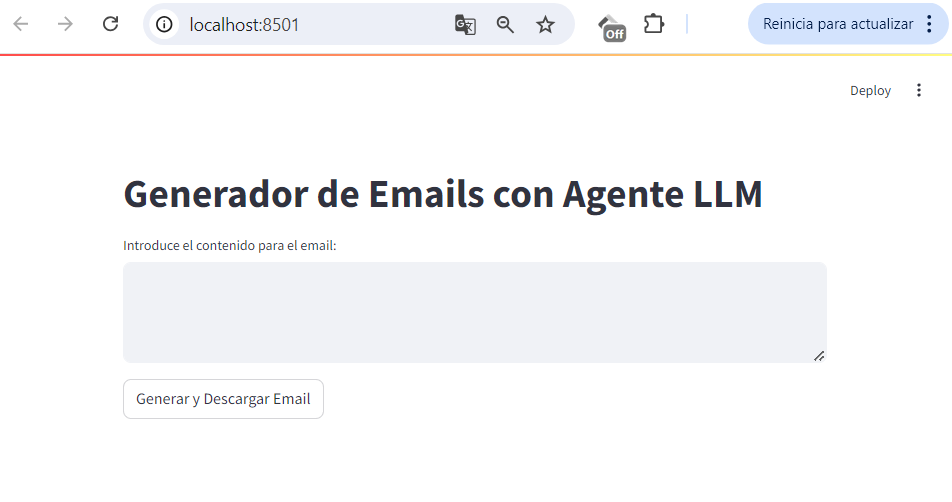
\includegraphics[width=1\linewidth]{Figures/interfaz_generador_email.png}
    \caption{Interfaz gráfica de la solución.}
    \label{fig:interfaz}
\end{figure}

La función principal en este proceso es la denominada \texttt{generar\_html\_y\_zip}. Dentro de esta se llama a la función \texttt{agent\_generate\_email} que es la que ejecuta el primer agente y desencadena todo el proceso hasta obtener el HTML final y las imágenes creadas. Posteriormente, utiliza la biblioteca zipfile para guardar el código HTML en un archivo \texttt{index.html} y para seleccionar las imágenes y encapsularlas en una carpeta \texttt{img}.

La funcionalidad de poder descargar un archivo ZIP es clave para este trabajo ya que es un requerimiento que el \textit{output} sea una carpeta que contenga la estructura de archivos necesaria para cargar el email en Adobe Campaign. Gracias a esta se logró un resultado acorde a lo que el cliente necesita.

%-------------------------------------------------------------------------------------------------------------
%-------------------------------------------------------------------------------------------------------------

\section{Integración de la solución}

En la figura~\ref{fig:diagrama_solucion} se puede observar un diagrama que resume todos los módulos que componen este trabajo y que hacen posible la generación de emails de forma automática. También se detalla el nombre del archivo .py donde se encuentra el código para cada parte.

\begin{figure}[!htpb]
    \centering
    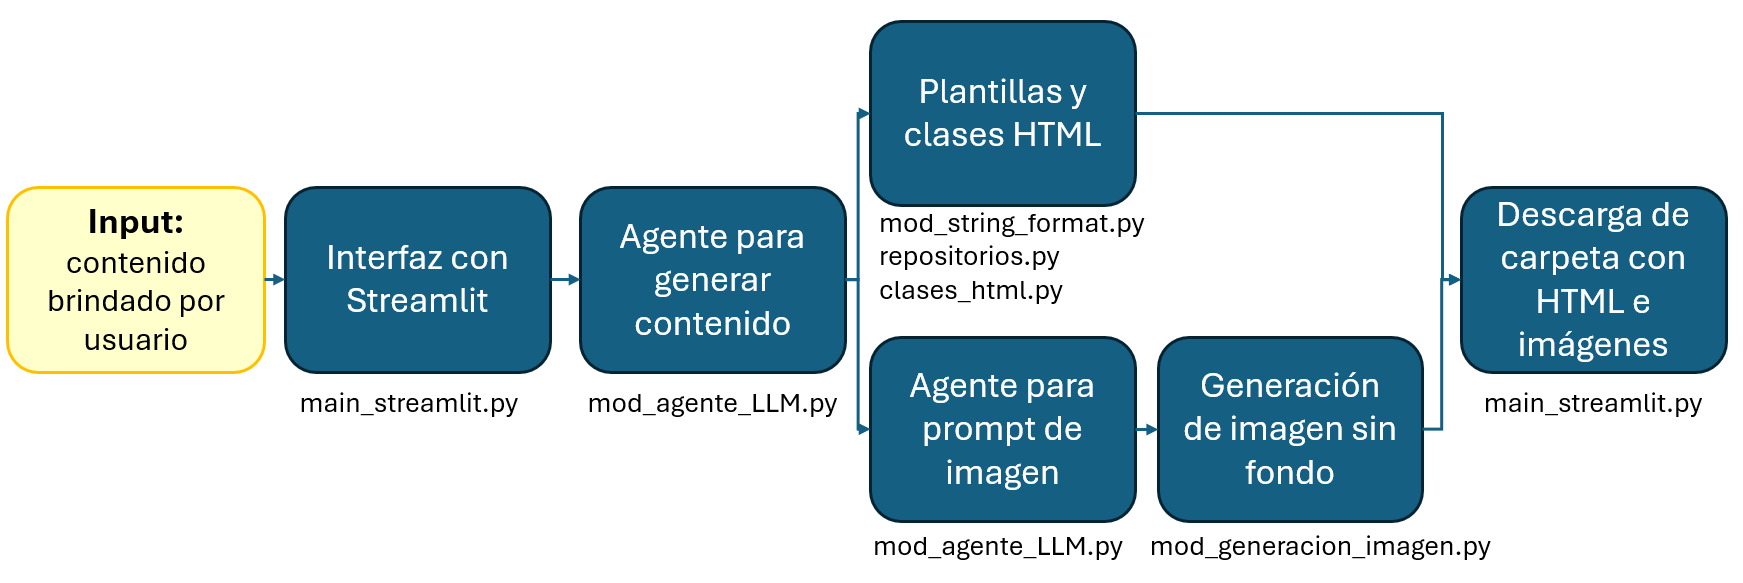
\includegraphics[width=\textwidth]{./Figures/diagrama_solucion_emails.png}
    \caption{Diagrama de la solución.}
    \label{fig:diagrama_solucion}
\end{figure}

Para recapitular lo explicado en las anteriores secciones, se puede resumir el proceso en las siguientes etapas:

\begin{itemize}
    \item El usuario utiliza la interfaz gráfica para enviar como \textit{input} el mensaje que quiere transmitir con el email, con todo el detalle que se quiere comunicar.
    \item Una vez que el usuario presiona el botón, se ejecuta una función que llama al primer agente LLM y le comparte el \textit{input}. 
    \item Este agente revisa el contenido y genera los elementos de texto del email (título, párrafo inicial, nombre de la imagen de cabecera, entre otros.). Posteriormente coloca estos componentes en \texttt{elementos\_str}, que es una variable de texto con formato JSON. Esta sirve de \textit{input} tanto para crear las clases HTML, como para generar la imagen de cabecera.
    \item La variable \texttt{elementos\_str} es decodificada y convertida en un diccionario de Python. Luego, cada elemento es asignado a la clase correspondiente. Finalmente todas las clases y elementos se utilizan para crear una instancia de la clase \texttt{Email\_HTML}. Se ejecuta el método \texttt{constructor\_html} de esta instancia para generar el HTML final.
    \item A su vez, la misma variable \texttt{elementos\_str} es enviada al siguiente agente LLM que analiza el contenido del email y crea un \textit{prompt} para generar la imagen de cabecera.
    \item Este \textit{prompt} se envía posteriormente a la función \texttt{generar\_imagen\_final} que engloba tanto la creación de la imagen en bruto, como la remoción del fondo.
    \item Finalmente, tanto el código HTML como las imágenes son guardados dentro de una carpeta comprimida que es descargada por el usuario.
\end{itemize}

Con este proceso se logra una integración fluida de todas las partes del sistema, lo que permite que los usuarios generen y descarguen emails personalizados y visualmente coherentes con facilidad.
